\chapter{Methodology}
\label{chap:2}
\ChapterPageStuff{2}

\section{Preamble}
In this chapter the methodology to create and implement a logging mechanism to do system utilisation analysis on software system will be discussed. In \Cref{sec:EventLogging} provided the needed literature to create a logging mechanism in \Cref{sec:Ch3_LoggingMechanism} for two software systems.

\section{Logging mechanism}\label{sec:Ch3_LoggingMechanism}
For this study two software systems are used to implement two different logging mechanisms. The first software system which will be called System A, is energy management system that uses \emph{PHP}. System B is a \emph{.NET Framework}\footnote{\label{ftn:NetFramework}\textbf{.NET Framework} is a run-time execution environment that consists of common language run-time (\emph{CLR}) and a \emph{.NET Framework Class Library} \cite{Harkness2007}.} system with a \emph{MVC} architecture as in \Cref{fig:ch2_Flow_MVC_Architecture} and is the administrative software system to configure System A.

\subsection{Logging points}
Logging point are essential data that describes the event's key features when creating a log as discussed in \Cref{sec:Ch1_LoggignPoints}. Both System A and B have certain key logging points that needs to be obtained from the user generated event.

\subsubsection{System A's logging points}
In \Cref{fig:ch2_SystemA_Dashboard} each mine group have multiple toolboxes linked to them. They can be same toolbox linked to both mine groups such as \emph{T1} and \emph{T3}. These toolboxes represent a group of dashboards related to the aspects of energy management of mines. Each of these toolboxes have a dashboards linked to them and each mine group can have different dashboards linked to the to the same toolbox. Each one of these mine groups, toolboxes and dashboards forms part of System A's web pages which the user can access where event logs are generated.

\begin{figure}[!htb] % An h :here, t: top, b: bottom.
	\centering % cent the figure
	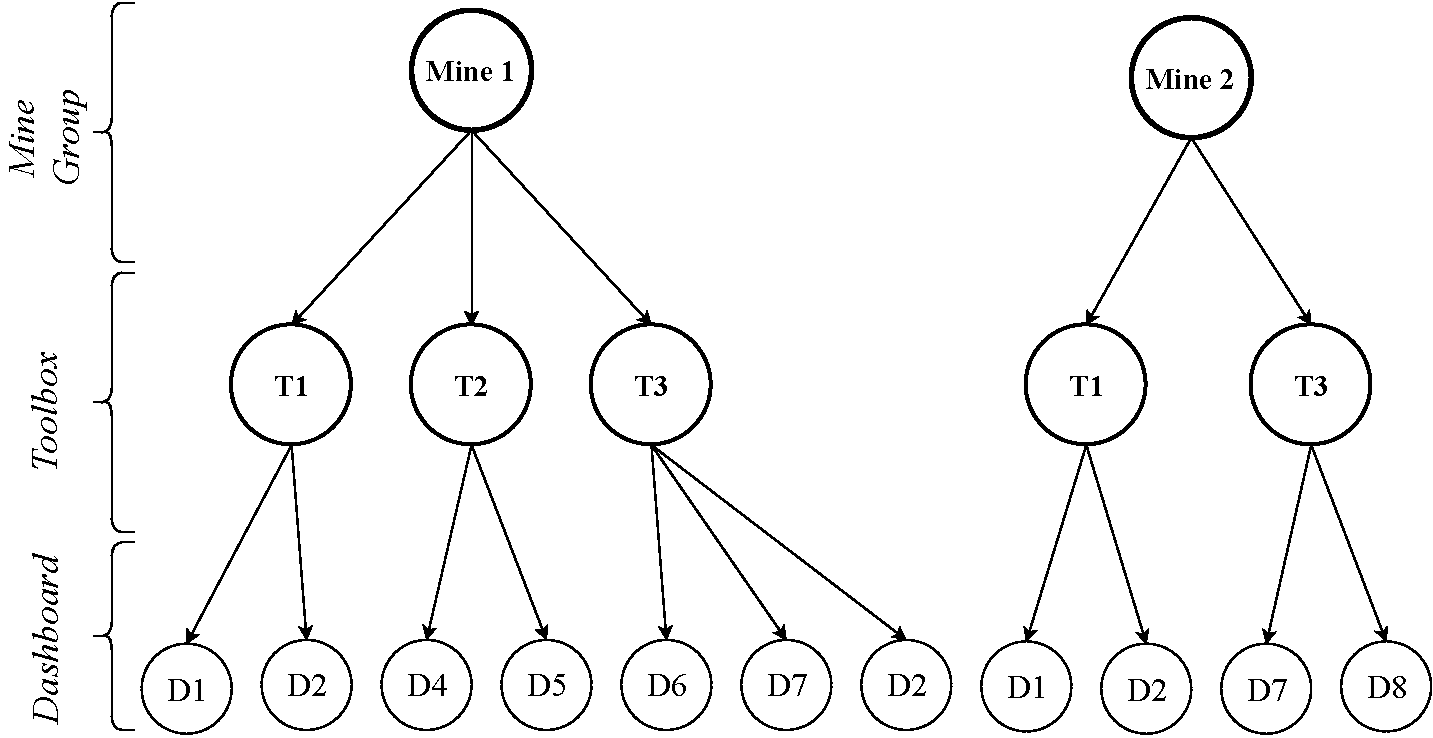
\includegraphics[width=0.9\textwidth]{Images/Chapter2/SystemA_Dashboard/SystemA_Dashboard.pdf}
	\caption[System A dashboard links]
	{\textit{System A dashboard links}}\label{fig:ch2_SystemA_Dashboard}
\end{figure}

The \emph{PHP} session helps to keep to track of any information needed for these pages to be fully functional like the user's identity and dashboard related data. This information can be used to give insight on which page the user is currently active on. In this case for System A the important \emph{PHP} session information is:

\begin{itemize}
	\item \textbf{User's identity:} The session contains the user's name and identity number which is the unique primary key for the user. This session information will always be available if the user is active on the software system from the instance they are logged in and verified until the user logs out and close their browser.
	\item \textbf{Group identity:} System A is used for multiple mine companies, each of the mining companies have a unique identity number. If a user is accessing on the dashboards, the group identity number is used to get 
	\item \textbf{Dashboard identity:} Each dashboard uses the \emph{PHP} files to construct a web page the user can view. To correctly navigate and get the correct page when the user request it, a unique identity number is used. In some cases for this system the same \emph{PHP} file can be used for multiple dashboards as extra configuration data is obtained from the database for that specific dashboard identity number.
	\item \textbf{Configuration meta data identity:} In \Cref{fig:ch2_SystemA_Dashboard} the same dashboard can be linked to different mine groups or toolboxes. The \emph{PHP} session contains any other identification parameters of which meta data should be loaded to configure the dashboard for the correct mine group and toolbox.
\end{itemize}

In \Cref{tbl:Ch2_PHP_LoggignMechanism} System A's key logging points which are saved in a \emph{SQL} database. These logging points have the essential data that is important to the event that is logged.

\begin{table}[!htb]
	\centering
	\small
	\caption[Logging points]
	{\textit{System A user activities table}}
	\label{tbl:Ch2_PHP_LoggignMechanism}
	\begin{threeparttable}
		\begin{tabularx}{\textwidth}{|l|l|X|}
			\hline \textbf{Column Name} & \textbf{SQL Data Type} & \textbf{Description} \\
			\hline \textbf{ActivityID} & INT(11) & The activity identification is a incremental number of the event that is logged.\\
			\hline \textbf{DashboardID} & DATETIME & Foreign reference key to the Dashboard table.\\
			\hline \textbf{UserID} & VARCHAR(45) & Each user has a unique identifier which is a numerical identification number that is foreign key reference to the User table.\\
			\hline \textbf{GroupID} & INT(4) & This foreign key reference to the Group table is contract groups identification number. \\ 
			\hline \textbf{Timestamp} & DATETIME & This is the time which the event took place.\\			
			\hline \textbf{ActivityType} & ENUM\tnote{*} & Each event that user initiated has an activity type. \\
			\hline \textbf{File} & VARCHAR(200) & This the \emph{PHP} file from which the request is processed.\\
			\hline \textbf{RequestParameters} & JSON & Request parameters of the event. \\
			\hline
		\end{tabularx}
		\begin{tablenotes}
			\item[*] ENUM have the values Dash, Report and DetailView.
		\end{tablenotes}
	\end{threeparttable}
\end{table}

\begin{figure}[!htb] % An h :here, t: top, b: bottom.
	\centering % cent the figure
	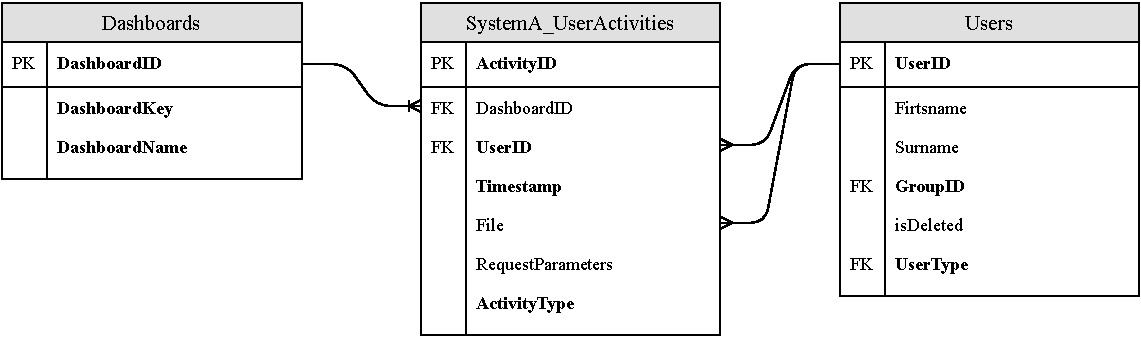
\includegraphics[width=0.95\textwidth]{Images/Chapter2/SystemA_ERD_Basic/SystemA_ERD_Basic.pdf}
	\caption[System A user activity ERD]
	{\textit{System A user activity ERD}}\label{fig:SystemA_Basic_ERD}
\end{figure}

\clearpage

\subsection{System A logging mechanism design}

In \Cref{fig:ch2_SystemA_Arch_Design} is the design for the System A's logging mechanism that consist of two different operations two log the event data that is generated from the user. These two main operations are used based on where the event is generated from either the PHP or MVC software components. The logging mechanism consist of two main functional requirements (\textbf{F/R}) that two main operations will use.

\begin{figure}[!htb] % An h :here, t: top, b: bottom.
	\centering % cent the figure
	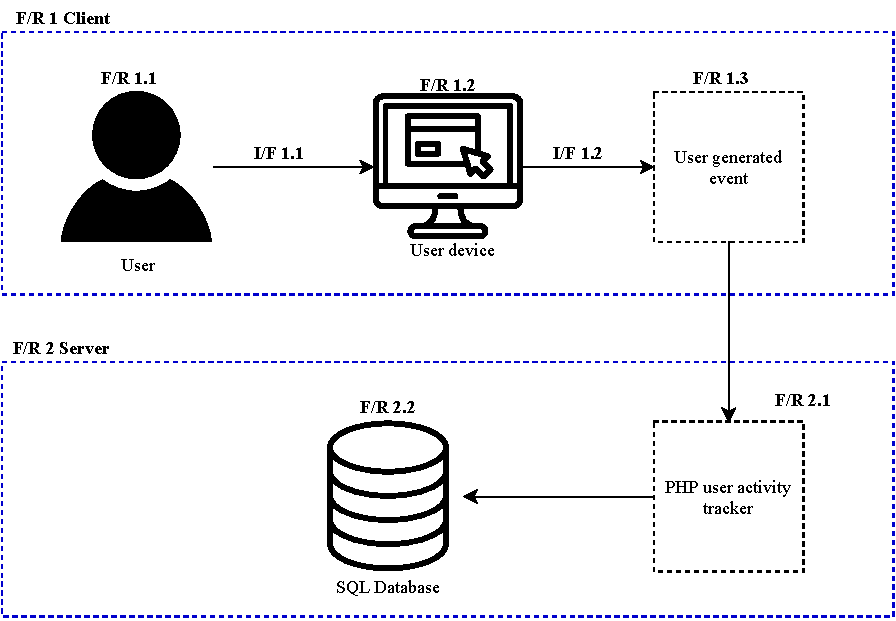
\includegraphics[width=0.99\textwidth]{Images/Chapter2/SystemA_Architecture_Diagram/SystemA_Architecture_Diagram.pdf}
	\caption[System A logging mechanism architecture design]
	{\textit{System A logging mechanism architecture design}}\label{fig:ch2_SystemA_Arch_Design}
\end{figure}

\textbf{F/R 1} of \Cref{fig:ch2_SystemA_Arch_Design} is the client side of the logging mechanism of System A.

\begin{table}[!htb]
	\centering
	\small
	\caption[System A's logging mechanism sub-systems]
	{\textit{System A's logging mechanism sub-systems}}
	\label{tbl:ch2_SystemA_SubSystems}
	\begin{tabularx}{\textwidth}{|l|X|}
		\hline \textbf{F/R 1.1} & The user \\
		\hline
	\end{tabularx}
\end{table}

\clearpage

\begin{figure}[!htb] % An h :here, t: top, b: bottom.
	\centering % cent the figure
	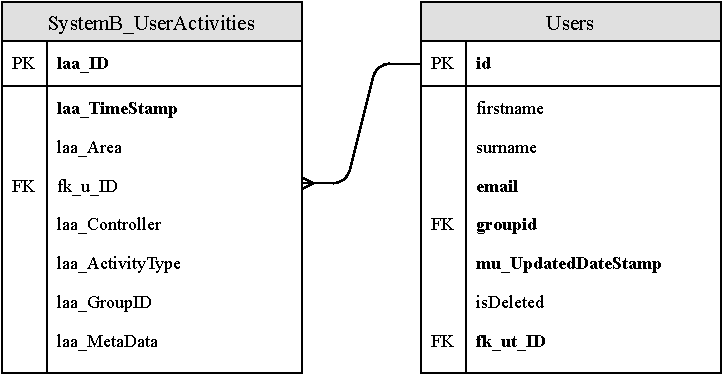
\includegraphics[width=0.9\textwidth]{Images/Chapter2/SystemB_ERD_Basic/SystemB_ERD_Basic.pdf}
	\caption[System B user activity ERD]
	{\textit{System B user activity ERD}}\label{fig:ch2_SystemB_Basic_ERD}
\end{figure}

\begin{figure}[!htb] % An h :here, t: top, b: bottom.
	\centering % cent the figure
	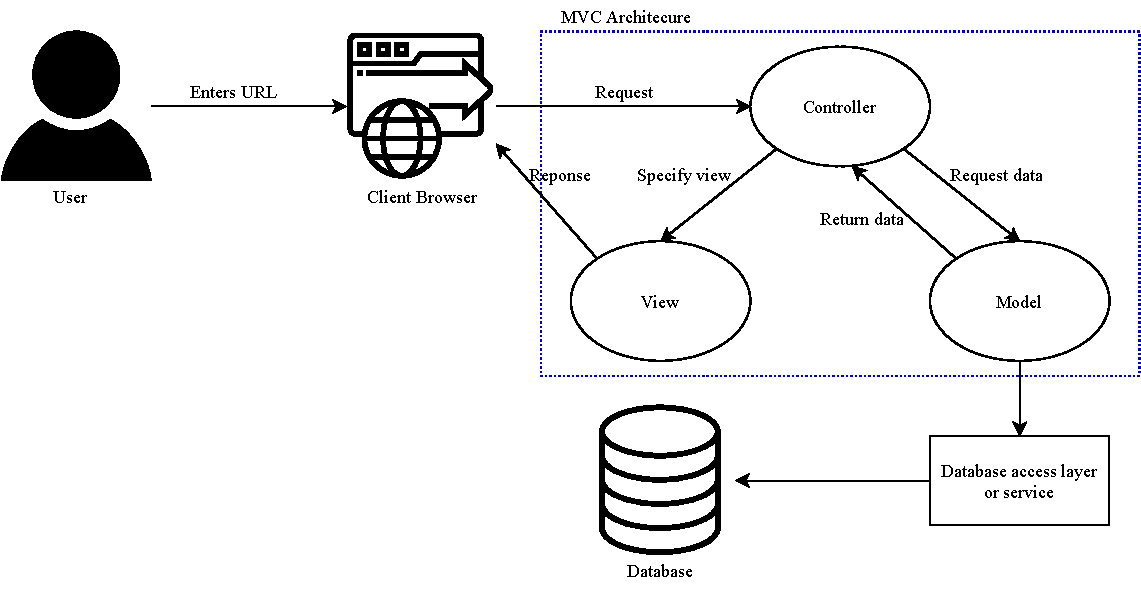
\includegraphics[width=0.95\textwidth]{Images/Chapter2/Flow_MVC_Architecture/Flow_MVC_Architecture.pdf}
	\caption[Request flow in MVC architecture]
	{\textit{Request flow in MVC architecture \cite{Gu2010}}}\label{fig:ch2_Flow_MVC_Architecture}
\end{figure}

\subsection{Logging mechanism}

\section{System utilisation analysis}

\section{Integration}
In this section the integration of the utilisation analysis and logging mechanism will be discussed.

\section{Conclusion}
Conclude the chapter about the development of the logging mechanism and utilisation analysis.